\chapter{Architecture}


\section{Proposed Architecture}
\subsection{Introduction}
In this project we will be designing the architecture for our game, and it’s achieved by using lucidchart for UML diagram drawing.
The reason for choosing this tool, simply because it have those necessary symbols already predefined, it also gives us the ability to work on diagrams collaboratively. We will be using UML 2.X specification.

\subsection{Abstract System Architecture Overview}
An abstract UML class diagram is provided as Figure~\ref{fig:classdiagram}
\begin{figure}[h]
	\begin{centering}
		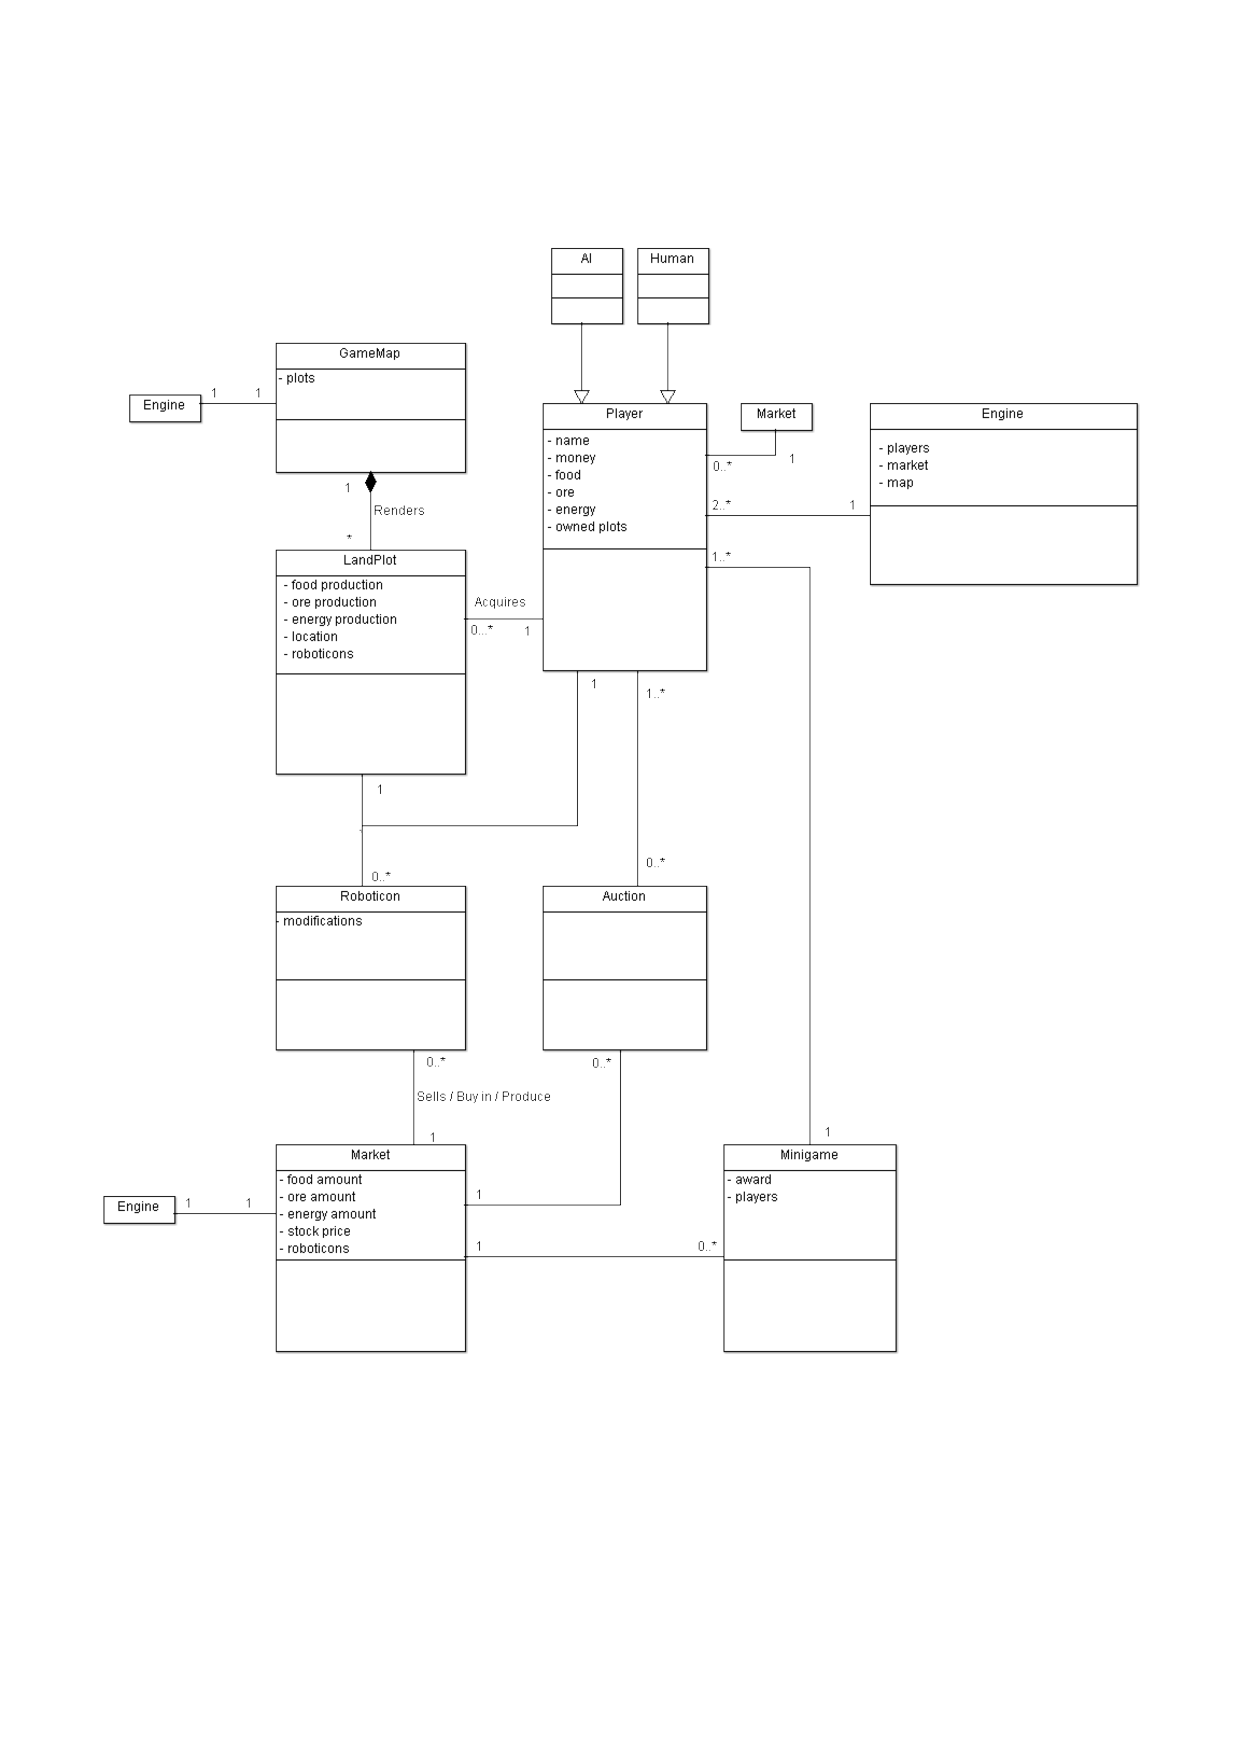
\includegraphics{AbstractDiagram.pdf}
		\caption{Abstract UML class diagram showing the relationships between classes in the software}
		\label{fig:classdiagram}
	\end{centering}
\end{figure}

\subsection{Entities}
We have identified the following classes that will be used in our system: \\

\begin{tabular}{|l|p{13cm}|}
	\hline
	Engine & The game engine itself, in charge of communications between classes. \\ \hline
	Player & The player entity has 2 child classes - AI and Human. Both have same base method and property names, with some different method bodies. \\ \hline
	LandPlot & Each instance of this class will represent a single tile on the map \\ \hline
	GameMap & This class is controlled directly from the engine. It stores all “LandPlot” instances. \\ \hline
	Roboticon & Roboticon is used in LandPlot for resource generation, trade between the player and the market. \\ \hline
	Market &The trading center. Players can buy or sell different types of resources and roboticons. It connects with the minigame class. \\ \hline
	Minigame & This class content a minigame for gambling, it is connected to the Market. \\ \hline
	Auction & The auction system, each instance will handle an individual auction that involves specific or selected players. \\ \hline
	
\end{tabular}

\subsection{Collaboration Diagrams}
These are collaboration diagrams which show how the classes in our game will interact to complete various tasks.
They also allowed us to test our class diagram and ensure that all necessary relationships had been established.
They are provided as Figures~\ref{fig:collab1}~to~\ref{fig:collab8}.

\begin{figure}[h]
	\begin{centering}
		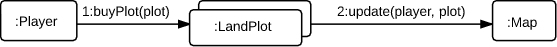
\includegraphics[width=\textwidth]{figures/collab1.png}
		\caption{Collaboration Diagram: Buying a plot of land}
		\label{fig:collab1}
	\end{centering}
\end{figure}
\begin{figure}
	\begin{centering}
		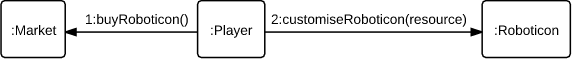
\includegraphics[width=\textwidth]{figures/collab2.png}
		\caption{Collaboration Diagram: Buying/Customising Roboticon from Market}
		\label{fig:collab2}
	\end{centering}
\end{figure}
\begin{figure}
	\begin{centering}
		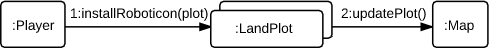
\includegraphics[width=\textwidth]{figures/collab3.png}
		\caption{Collaboration Diagram: Roboticon Installation}
		\label{fig:collab3}
	\end{centering}
\end{figure}
\begin{figure}
	\begin{centering}
		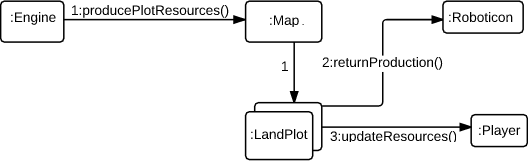
\includegraphics[width=\textwidth]{figures/collab4.png}
		\caption{Collaboration Diagram: Production of Resources}
		\label{fig:collab4}
	\end{centering}
\end{figure}
\begin{figure}
	\begin{centering}
		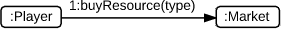
\includegraphics[]{figures/collab5.png}
		\caption{Collaboration Diagram: Buying from Market}
		\label{fig:collab5}
	\end{centering}
\end{figure}
\begin{figure}
	\begin{centering}
		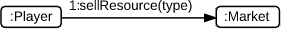
\includegraphics[]{figures/collab6.png}
		\caption{Collaboration Diagram: Selling to Market}
		\label{fig:collab6}
	\end{centering}
\end{figure}
\begin{figure}
	\begin{centering}
		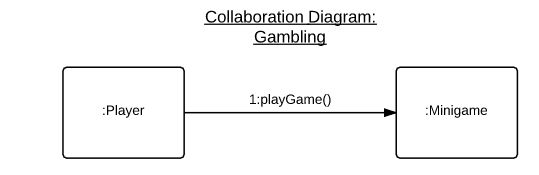
\includegraphics[]{figures/collab7.png}
		\caption{Collaboration Diagram: Gambling}
		\label{fig:collab7}
	\end{centering}
\end{figure}
\begin{figure}
	\begin{centering}
		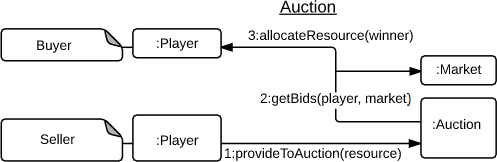
\includegraphics[width=\textwidth]{figures/collab8.png}
		\caption{Collaboration Diagram: Auction}
		\label{fig:collab8}
	\end{centering}
\end{figure}


\section{Systematic Justification of Architecture}
Designing an abstract representation of the system architecture required a lot of thought from the team, as it is easy to overlook important relationships between classes and objects.
We began the design process by looking through the brief and our requirements document and creating a list of classes that we felt encompassed the fundamental game elements.
From this process, we came up with the entities shown in the table above.
Below is a description of how each class will work and justification for why it will work that way.

\subsection{Engine}
The game engine is a particularly important class, as it is responsible for initiating and controlling each phase of the game, as well as invoking random events which will affect the game’s current state. In order for the Engine to be able to do this, it must be able to communicate with the other fundamental classes, these being the GameMap and each instance of the Player class.
From the brief, we established that there is a one-to-one relationship between the Engine and the GameMap, and a one-to-many relationship between the Engine and the Player (we have set the number of instances of player to be two at the moment). The Engine doesn’t need to be connected to other classes such as the Market and the LandPlot as these can be accessed via GameMap and Player.
We chose not to give many classes a relationship with the Engine, as this will create too many class couplings, meaning that if we need to make changes in the Engine class, changes will need to be made in many other classes too.

\subsection{Player}
The player class models each player in the game, and the set of decisions that they can make while playing.
These decisions include: buying plots of land, installing roboticons on plots, buying and selling from the market, and gambling in the bar (as detailed throughout the requirement section).
Because of the player’s large range of actions in the game, we needed the player to have relationships with quite a few of the other classes, including the Market, the Auction, various instances of the LandPlot class, and the Minigame.
Although this may seem risky due to the slightly monolithic nature of the class, we feel that the only way we can deliver a piece of software which satisfies all of the requirements is to design the system in this way.
The Player class will be the parent of two other classes called Human and AI.
These classes will inherit the attributes and methods of player, but will overwrite methods to suit each player role.
The player will have attributes detailing the name of the player, as well as the amount of money they have, the number of each resource they own (food, energy, ore), and the plots they own.

\subsection{Roboticon}
The roboticon class is responsible for production of resources on a plot, as stated in requirement 7.1.1., and any modifiers that will be applied to the rate of production.
It is therefore necessary for a roboticon to be able to communicate with the land plot on which it is placed.
In accordance with requirements 6.1.4. and 6.1.5. the player will be able to customise the roboticon by installing upgrades for money.
Finally the roboticon is produced, stored, and sold by the market so the classes must be able to communicate, as described in requirements 6.1.1 and 6.1.2..
It will have attributes to determine how it will alter the production of resources on a plot.

\subsection{Market}
The Market is the class responsible for managing the price of resources in the game (based on supply and demand), and also producing roboticons, as specified in requirement 8.1.2..
The player can directly buy and sell resources to/from the market so must be able to interact with it.
The market will also engage in the auction, placing bids against the other player and affecting the price at which resources are bought and sold. It will therefore interact with the auction.
The market also has a relationship with roboticons as it can buy sell and produce them.

\subsection{Minigame}
The minigame is a fairly simple class as it only interacts with the player.
The minigame is a game found in the market which will allow the player to gamble and either gain or loses money which will satisfy requirement 9.1.1.

\subsection{Auction}
The Auction Class is responsible for players buying and selling resources to each other, as described in requirement 8.1.1.
The market will also act as a bidder in the auction giving bids based on the supply/demand of the resource allowing access to the auction in a 2 player Game.
The auction will take resources to be sold from one player and bids from the other player(s) and the market, then provide the resources to the highest bidder.

\subsection{LandPlot}
The LandPlot class is used for purchase, resource production and customisation as Player request as described in requirement 2, 7.1.3 and 3.1.1.
All LandPlots instances are stored inside the GameMap class for rendering, and those LandPlots shall have the same size as described in requirement 1.2.2.
On the occurrence of random event, the production rate for different resources should change respectively if criteria matches per requirement 2.2.2. 

\subsection{GameMap}
The GameMap Class is in charge of storing all instances of LandPlot and the interaction with the Engine to render the Game Map to the screen.
At beginning of the game, GameMap will initialise and set all LandPlots to a state of “unoccupied” to allow the Player to view and purchase as described on requirement 1.1.1 and 2.2.3.

